\documentclass[a4paper,11pt]{scrartcl}
\usepackage{fullpage}

\usepackage[english]{babel}
\usepackage[utf8]{inputenc}

\usepackage[version=4]{mhchem}

\usepackage{siunitx}
\usepackage{graphicx}
\usepackage{commath}
\usepackage[retainorgcmds]{IEEEtrantools}

\newcommand*{\Li}{\ce{Li}}
\newcommand*{\n}{n_{\Li}}
\newcommand*{\nv}{\hat{n}}
\newcommand*{\pn}{\frac{\partial{}\n}{\partial{}t}}
\newcommand*{\F}{\mathcal{F}}
\newcommand*{\dv}[1]{\nabla\cdot\left({#1}\right)}
\newcommand*{\dx}{\dif{}x}
\newcommand*{\I}[1]{\int_{\Omega}{#1}\dx}
\newcommand*{\Ib}[1]{\int_{\partial \Omega}{#1}\dx}
\newcommand*{\Dt}{\Delta t}
\newcommand*{\Po}{\Phi_{\text{contact}}^{\text{ohmic}}}


\begin{document}
\begin{figure}[h]
\centering
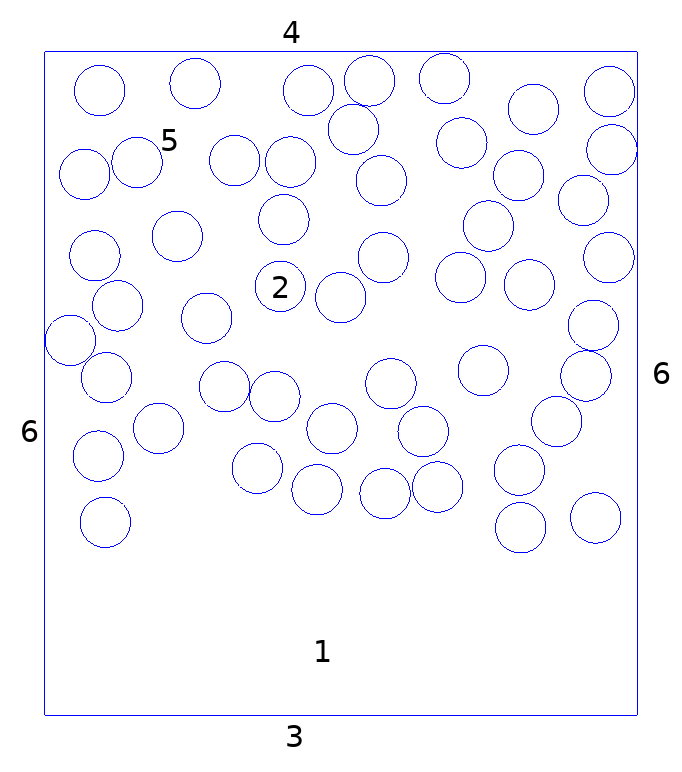
\includegraphics[width=0.5\linewidth]{pic/geometry.png}
\end{figure}

\section*{Model Equations}
Taken from~\cite{garcia05}:
\begin{IEEEeqnarray*}{cc}
 1\&2 & \left\{\begin{aligned}\pn = \dv{D(\n) \nabla \n} +
  \dv{\frac{D(\n) z(x) \F \n}{R T} \nabla \phi} \\
0 = \frac{\partial\rho}{\partial{}t} =
  \dv{\kappa_T(x) \nabla \phi} + \dv{\frac{D(\n) z(x) \F \n}{R T} \nabla \n} \\
  \end{aligned}\right. \\
  3\&5 & J \cdot \nv = i_0(\n) \frac{(\alpha_a + \alpha_c) \F \eta_e(\phi, \n)}{RT}
  \\
  3 & N^0_{\Li} = \frac{I_0}{A \F} \\
  4 &\left\{\begin{aligned}J \cdot \nv_c = - \frac{I_0}{A} \\ N_{\Li} \cdot \nv_c = 0\end{aligned}\right.\\
  6 & \left\{\begin{aligned}J \cdot \nv = 0 \\ N_{\Li} \cdot \nv = 0\end{aligned}\right.
\end{IEEEeqnarray*}

Further relations and equations:
\[J = \kappa E = - \kappa \nabla \phi\]
\[D_{\Li} = D_{\Li}^*\left(1+\frac{\partial{}\ln{\gamma_{\Li}}}{\partial{}\ln{\n}}\right)\]
\[i_0(\n) = \F k_r (n_s - \n)^{\alpha_a}(\n)^{\alpha_c}\]
\[\eta_e = E \cdot \delta - \left[ U(\n) - \Po \right]\]
\[\Po = R_cI_0\]

\subsection*{Open-circuit potentials}
\begin{itemize}
  \item \ce{Li_yMn_2O_4} equation (A-1) from~\cite{doyle95} Appendix 3-A.
    \begin{IEEEeqnarray*}{rCl}
      U(y) &=& 4.19829 + 0.0565661 \tanh{[-14.5546 y + 8.60942]} \\
      &-& 0.0275479 \left[ \frac{1}{(0.998432-y)0.492465}-1.90111 \right]\\
      &-& 0.157123 \exp{(-0.04738 y^8)} + 0.810239 \exp{[-40(y-0.133875)]}
      \qquad 0 \leq y \leq 1.0 \\
    \end{IEEEeqnarray*}

  \item \ce{Li_xC_6} equation (A-2) from~\cite{doyle95} Appendix 3-A.
    \[ U(x) = -0.16 + 1.32 \exp{(-3.0 x)}, \quad 0 \leq x \leq 0.7\]

\end{itemize}

\section*{Variational Formulation}

\begin{IEEEeqnarray*}{rCl}
  \I{\pn v} &=& \I{\dv{D(\n) \nabla \n} v}
  +\I{\dv{\frac{D(\n) z(x) \F \n}{RT} \nabla \phi} v} \\
&=& -\I{D(\n) \nabla \n \cdot \nabla v} + \Ib{D(\n)(\nabla\n \cdot \nv) v} \\
&&-\I{\frac{D(\n) z(x) \F \n}{R T} \nabla \phi \cdot \nabla v}
+\Ib{\left(\frac{D(\n) z(x) \F \n}{R T} \nabla \phi \cdot \nv\right) v} \\
&=& -\I{D(\n) \nabla \n \cdot \nabla v}
+ \int_{\partial\Omega_{3}}{D(\n)\left(\frac{I_0}{A\F n_T}\right) v}\dx \\
&&-\I{\frac{D(\n) z(x) \F \n}{R T} \nabla \phi \cdot \nabla v} \\
&&-\int_{\partial\Omega_{3,5}}{i_0(\n) (\alpha_a+\alpha_c)\eta_e(\phi,\n)
  \frac{D(\n) z(x) \F^2 \n}{R^2 T^2 \kappa_T(x)}} v \dx \\
&&+\int_{\partial\Omega_4}{\frac{D(\n) z(x) \F \n I_0}{R T \kappa_T(x) A} v} \dx \\
\end{IEEEeqnarray*}

\begin{IEEEeqnarray*}{rCl}
0 &=& - \I{\kappa_T(x) \nabla \phi \cdot \nabla \psi} +
\Ib{(\kappa_T(x) \nabla \phi \cdot \nv) \psi} \\
&& - \I{\frac{D(\n) z(x) \F \n}{R T} \nabla \n \cdot \nabla \psi} +
\Ib{\left(\frac{D(\n) z(x) \F \n}{R T} \nabla \n \cdot \hat{n}\right) \psi} \\
&=& - \I{\kappa_T(x) \nabla \phi \cdot \nabla \psi}
-\int_{\partial\Omega_{3,5}} i_0(\n) \frac{(\alpha_a+\alpha_c)\F\eta_e(\phi,\n)}{RT}\psi \dx \\
&& +\int_{\partial\Omega_4} \frac{I_0}{A\kappa_T}\psi \dx \\
&& - \I{\frac{D(\n) z(x) \F \n}{R T} \nabla \n \cdot \nabla \psi}
+ \int_{\partial\Omega_{3}}{\frac{D(\n)I_0 z(x) \F \n}{RTA\F n_T} \psi}\dx \\
\end{IEEEeqnarray*}


\section*{Time Stepping}
We write our system in a shorter form:
\begin{IEEEeqnarray*}{rCl}
n_t &=& f(n) + g(n) \phi \\
0  &=& A \phi + h(n)
\end{IEEEeqnarray*}
We first try the Crank-Nicolson method, because it is unconditionally stable.
Another choice would be the implicit Euler method.
\begin{IEEEeqnarray*}{rCl}
\frac{n(t+\Dt)-n(t)}{\Dt} &=& \frac{1}{2}(f(n(t+\Dt)) + g(n(t+\Dt))\phi(t+\Dt) +
f(n(t))+g(n(t))\phi(t)) \\
0 &=& \frac{1}{2}\left(A \phi(t+\Dt) + h(n(t+\Dt)) + A\phi(t) + h(n(t))\right)
\end{IEEEeqnarray*}

One way to solve the system would be to eliminate $\phi(t+\Dt)$ by
rearranging the second equation
  \[\phi(t+\Dt) = - A^{-1} h(n(t+\Dt)) - \phi(t) - h(n(t))\]
and then plugging that into the first equation.

\section*{Parameters and Constants}

\begin{tabular}{c|c|c|c}
  Symbol & Name & Value & Unit \\
 \hline
  $\F$ & Faraday constant & \num{96485.33289} & \si{\coulomb  \mol^{-1}}\\
  $R$ & molar gas constant & \num{8.3144598} & \si{\J \K^{-1} \mol^{-1}}\\
 \hline
  $D_{m}$ & diffusivity of electrolyte/carbon mixture & \num{2.66e-5}& \si{\cm^2\s^{-1}} \\
  $D_{p}$ & diffusivity of \ce{Li_yMn_2O_4} particles & \num{1e-9}& \si{\cm^2\s^{-1}} \\
  $\kappa_{T, m}$ & electric conductivity of electrolyte/carbon mixture & \num{2.53e-2} & \si{\siemens\cm^{-1}}\\
  $\kappa_{T, p}$ & electric conductivity of \ce{Li_yMn_2O_4} particles & \num{3.8e-2} & \si{\siemens\cm^{-1}}\\
  $T$ & absolute temperature & \num{298.15} & \si{\K} \\
  $n_T$ & normalization concentration value for lithium & \num{22.86} & \si{\mol\dm^{-3}} \\
  $\alpha_a$ & anodic empirical constant & \num{0.5} & \\
  $\alpha_c$ & cathodic empirical constant & \num{0.5} & \\
  $A$ & battery cross-sectional area & \num{24.0} & \si{\cm^2} \\
  $k_r$ & reaction rate constant at particle/electrolyte interface & \num{24.0} & \si{\cm^2} \\
  & battery capacity & \num{2} & \si{\mA\hour\cm^{-2}} \\
  $n_s$ & solubility limit of lithium in the electrode & ? & \si{\mol} \\
  $\delta_a$ & anode thickness & \num{250} & \si{\um} \\
  $\delta_c$ & cathode thickness & \num{174} & \si{\um} \\
  $\delta_s$ & separator thickness & \num{50} & \si{\um} \\
  $R_c$ & total electrode contact resistance & \num{2e-3} & \si{\ohm} \\
 \hline
  $n_0^a$ & normalized initial concentration of lithium in anode & \num{0.72} & \\
  $\phi_0$ & initial electric potential in cathode & \num{4.2} & \si{\V} \\
\end{tabular}

$I_0$ discharge current some multiple of battery capacity \si{\mA\hour}

\section*{Notes}
\begin{itemize}
\item Don't forget normalizing $\Li$ boundary conditions.
\end{itemize}
\section*{Questions}
\begin{itemize}
\item Activity coefficient?

  There's a difference between molal and molar coefficient! Which one is applicable?
  See~\cite{doyle95} chapter 4.
  They also used idealized versions, because measurement is hard.
  Also in~\cite{garcia05} they mention, that for pure and dilute compositions
  the activity coefficient satisfies Raoult's and Henry's law.

\item How to incorporate boundary conditions into time stepping?

  They are part of the (non-)linear functions $f, g, A, h$.

\item Are the functions dependent on the $\Li$ concentration dependent on the
  relative or absolute concentration? Which units?

  Probably absolute. Molar concentrations maybe.

\item The open-circuit potentials are they with molar concentrations?

  Unsure because of the \ce{Li_yMn_2O_4} notation and saying that $y$ is the
  parameter for the potential. It ranges from 0.0 to 1.0.

\item On boundaries $\partial\Omega_{3,5}$ is $z(x) = 0$ or $1$?

  Probably $1$, because otherwise the whole boundary condition would never
  have an influence.

\item What is porosity $\epsilon$ in~\cite{garcia05} Table II?

\item How big is the process zone $\boldsymbol{\delta} = \delta \boldsymbol{\hat{n}}$?

  For now take it as $\delta_a$ for boundary condition 3 and the radius of the
  particle for boundary condition 5.

\item Should we use Butler-Volmer relation instead of linearized version?
  Or stated differently: Is $|\F \eta_e R T| \ll 1$?

\item Do we need the equations for the anode?

  Probably yes, because the Butler-Volmer relation needs to now the potential
  and concentration in the anode.

\item What is the reaction rate constant at the anode/electrolyte interface?

\item What is the solubility limit of lithium $n_s$ in the electrodes?

  Maybe one if we use relative concentration. Or depending on electrode, because
  open circuit potential for \ce{Li_xC_6} is 0 at ~0.7 in graph from~\cite{doyle95} Appendix 2-A.

\item Which open-circuit potentials should we use? Appendix 2-A or 3-A?

\item What are the initial conditions in the electrolyte?

\end{itemize}

\bibliography{model}{}
\bibliographystyle{alpha}


\end{document}